\documentclass{sig-alternate-05-2015}

\usepackage[T1]{fontenc}
\usepackage{polyglossia}
\setdefaultlanguage{english}
\usepackage{csquotes}

\usepackage{fontspec}
\usepackage{xltxtra}
%\usepackage{libertine}

\usepackage[usenames, dvipsnames]{xcolor}
\graphicspath{{./img/}}

\usepackage[backend=biber, style=numeric]{biblatex}\bibliography{literatur.bib}

\usepackage{subcaption}
\usepackage{fancyref}

\usepackage[%
unicode=true,%
colorlinks=true,%
linkcolor=black,%
urlcolor=MidnightBlue,%
citecolor=black,%
filecolor=black%
]
{hyperref}


\newcommand{\todo}[1]{\textcolor{Red}{#1}}
\newcommand{\sebastian}[1]{\textcolor{Green}{#1}}
\newcommand{\stefan}[1]{\textcolor{BurntOrange}{#1}}
\newcommand{\etal}{\textit{et. al.}}
\newcommand{\Gray}[1]{\textcolor{Gray}{#1}}

\begin{document}

\conferenceinfo{IntSim}{2015, Augsburg}
\title{
Interactive Simulation WS 15/16\\ %
Project Report
}
\subtitle{EYES - Exchange Your Vision Simulator}
\numberofauthors{2}
\author{
% 1st. author
\alignauthor
Sebastian Lemp\\
%       \affaddr{Street, House}\\
%       \affaddr{PLZ City}\\
       \affaddr{University of Augsburg}\\
       \email{sebastian.lemp@student.uni-augsburg.de}
% 2nd. author
\alignauthor
Stefan Büttner\\
%       \affaddr{Street, House}\\
%       \affaddr{PLZ City}\\
       \affaddr{University of Augsburg}\\
       \email{stefan.buettner@student.uni-augsburg.de}
}
%\additionalauthors{Additional Authors}

% The date is actually not used in the acm template
\date{University of Augsburg, \today}

% Not neede for our purposes
%\terms{Terms}
%\keywords{Keyword 1, Keyword 2}
%% A category with the (minimum) three required fields
%\category{H.4}{Information Systems Applications}{Miscellaneous}
%%A category including the fourth, optional field follows...
%\category{D.2.8}{Software Engineering}{Metrics}[complexity measures, performance measures]

%% For the ACM ToG format
%\acmformat{ACMFormat}
%\acmVolume{Vol.}
%\acmNumber{Nr.}
%\acmYear{YYYY}
%\acmMonth{MM}
%\acmArticleNum{XXX}
%\doi{DOI}


\maketitle
\begin{abstract}
Many diseases can be treated well if recognized early.
This is also true for eye diseases.
So the point of the program presented in this paper is to let the user experience different kinds of eye diseases in order to show him warning signs and confront him with severe states of those diseases.
%That's why we want to inform the users about different eye diseases and their effects on the vision.
%That's why we built the EYES Simulator in combination with this paper.
In order to address especially a young audience, the presentation is in form of a small game developed in Unity3D.
The player will experience five different eye diseases in different levels in which he will go shopping and collect special items from his shopping list.
This scenario was chosen because we believe it to be a common, well known situation.
%We chose this scenario because everybody knows the situation.
In contrast to other eye disease simulators, which usually show the effects on static images, this one simulates colorblindness, glaucoma, cataract, and myopia/hyperopia interactivly.
This is achieved by implementing the diseases as image effects using CGI shaders.
%build up like an game where the player gets point for solving the task as fast as possible. Aswell the player should get the feeling of how difficult it can be living with one the the diseases.

\end{abstract}
% Disease list:
% -------------------------------------------------------------------------------
% (Stefan)     11 Disorders of sclera, cornea, iris and ciliary body
% (Sebastian)   1 Cataract (Grauer Star)
% (Stefan)      2 Retinal detachment and breaks
% (Sebastian)  14 Other retinal disorders
% (Stefan)      1 Glaucoma (Grüner Star)
% (Stefan)      2 Disorders of optic nerve and visual pathways
% (Sebastian)  10 Disorders of ocular muscles, binocular movement, accommodation and refraction
% (Stefan)      6 Visual disturbances and blindness
%              47

%
% Possible References:
% http://www.svi.cps.utexas.edu/EI466209.pdf

% http://www.icdvrat.org/2008/papers/ICDVRAT2008_S04_N06_Banks_McCrindle.pdf
%
% claim they have an real-time app for Android and iOS:
% http://www.brailleinstitute.org/sight-loss-blog/398-leading-eye-diseases.html 
%
% OpenGL real-time simulation
% http://percept.eecs.yorku.ca/papers/p127-vinnikov.pdf
% 

\section{Introduction}
Eye diseases have been an issue throughout all the human history.
In the beginning the focus layed on their treatment.
However, Virtual Reality (VR) is more and more pushing into the consumer market and could therefor be broadly used for education and thus prevention of eye diseases.
For example, the risk of suffering from retinal detachment can be greatly reduced if the signs are recognized early and a doctor is consulted.
Therefore, educational software can be used.
In addition, people would hopefully visit a doctor earlier if they already experienced a good simulation of a severe state of a disease, before they actually are in a severe state.
Other applications could be testing designs of consumer products like packaging or traffic signs or other signs at public places.

Although there are many simulations available already, they usually work on still 2D images, 2D video streams or static 3D scenes and don't have any game component.
Moreover, more sophisticated simulations are probably not easily available for public use and implementing a simulator using Unity3D in terms of an \emph{eye disease asset set} wrapped into a small game could be interesting for a broad audience.

So we implemented three visual disease simulators in Unity3D and applied them in a small game.
In this game the player has to collect items in a Supermarket, which is likely to be a well-known situation to everyone.

\section{Related Work}
There are different eye disease simulators available in the web already.
However, common ones, e.g. found on websites of health organizations, alter still 2D images and display them in the browser.
For example, the "Sehbehinderungs-Simulator" of ABSV~\cite{absv} lets the user choose from five different diseases: "Grauer Star" (Cataract), "Makula-Degeneration" (Macular degeneration), "Grüner Star" (Glaucoma), "Diabetische Retinopathie" (Diabetic retinopathy) and "Retinitis Pigmentosa" (Retinitis pigmentosa).
These you can test on different images like being at a crossraods, doing a puzzle or filling in a form. 
There are also real-time simulations available as described by Zhuming~\cite{eyediseasesim-zhuming} but the implementation is not available online.
\todo{Grammar:}They focusing a VR solution with common task in the household.

\section{Models and Methods}
%\begin{itemize}
%  \item Fulfill everyday tasks with impaired vision
%  \item Possible boni: 
%  \begin{itemize}
%    \item Get rid of disease by performing the right actions
%    e.g. take medication on the way or make a doctors appointment...
%    \item Preventive measures during the task to not get disease in next lvl
%  \end{itemize}
%  \item Target platform: Android \& Google Cardboard to address many people
%\end{itemize}

%Assets used: Standard Assets (Unity Technologies), Inventory Master - uGUI (Sander Buchheim), Supermarket Interior (FireMesh), Drag and Drop Pause Menu (Cinopt Studios)

The player is able to experience different types of eye diseases varying in severity. The game is set in a supermarket where the player has to shop for different objects. There are five different eye diseases to experience in five different levels.

\subsection{Gerneral game objects}

Each level has the same structure and the same target, its just different in what the Player has to pick up and which disease he got. He is able to Pause the game by pressing ESC, then the time stops and he cant move any longer. This was done with the "Drag and Drop Pause Menu" Asset. 

With the pause menu it is possible as well to End the game or jump back to the main menu.

\begin{figure}
    \centering
    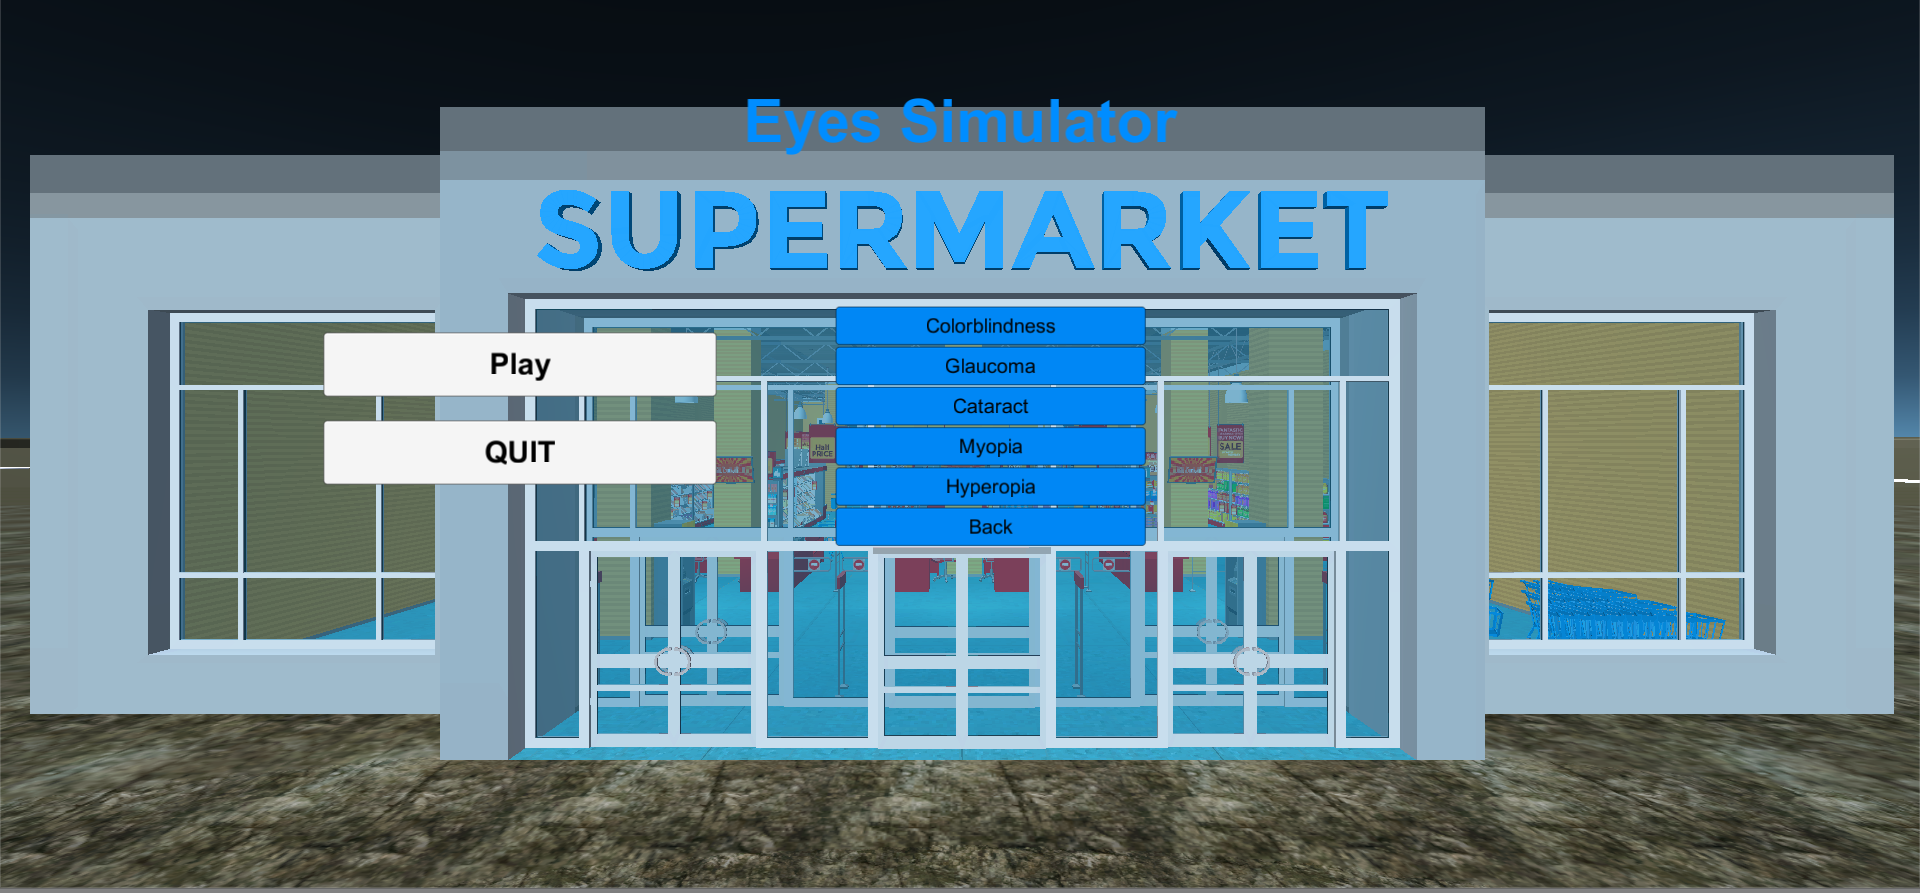
\includegraphics[width=\columnwidth]{Menu.png}
    \caption{Shows the Menu which the Player sees at the beginning.}
    \label{fig:menu}
\end{figure}

When the game starts the player is able to see a menu shown in \Fref{fig:menu}, like u can see he can press Play or Quit. After he hit the play button he can select between the different Eye diseases to start the level. The Quit button is to End the game. Each of levels got different eye disease witch makes it more difficult to finish the level. In all of the Level's the player is asked to collect different Items to finish his shopping list. The Player starts near the entrance of the shop as seen in \Fref{fig:gamestart}. You can see that in the left top corner a Text field with the instruction how he is able to move and operate. In the right top corner there is his shopping list to show which item he has to collect and bring to the till. He can walk with W,A,S,D through the shop and pick up different items like Milk or Bacon with pressing the E button. 

The jump function of the first person controller was disabled that the player cant jump on the shelves or over the counters.

\begin{figure}
    \centering
    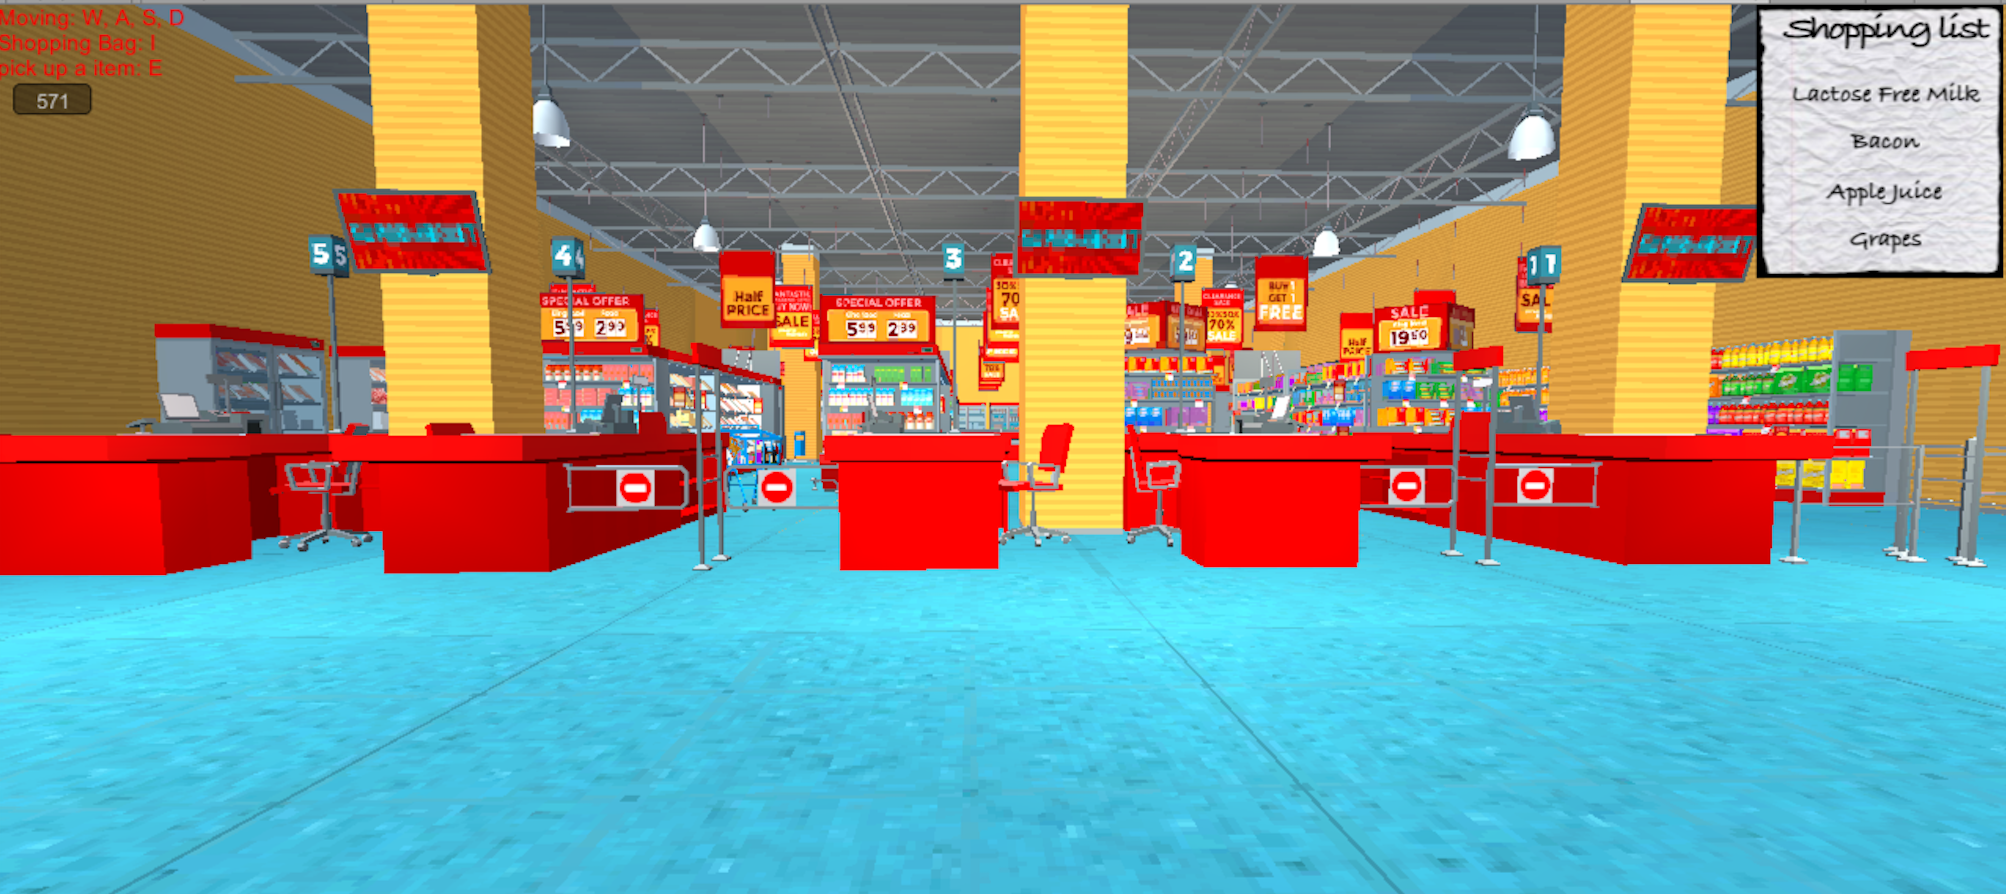
\includegraphics[width=\columnwidth]{Game.png}
    \caption{Gives an overview what the player sees when he selected a level.}
    \label{fig:gamestart}
\end{figure}

If the player press I a shopping bag appears where he can see what items he already picked up. Each items got a small description with some information about it, seen in \Fref{fig:ShoppingBag}. 

The Supermarket was build up with the "Supermarket Interior" Asset, there we added a first person controller and on every object colliders, that its not possible to walk through the objects. As well we reworked all items in the supermarket shelfs, that in every shelf is just one item type. This was made to make it not to difficult witch item should get picked uped. All Items where added to a Database which comes with the "Inventory Master" Asset. All items got a pick up script that its possible to collect them. We decided to put just one item with pick up script in the shelf that it is not possible to clear the hole racks.

In the Database we added the items and some small description. We choose nearly similar mesh like a milk bottle with a red lid and a bottle with a white lid, to show the problems of a person with color blindness.

The Shopping list was just done with a separate Canvas, in the left top corner, with a text field to show the task to the PLayer. Aswell we put a image on it that it looks like an usual crumpled shopping list. 

\begin{figure}
    \centering
    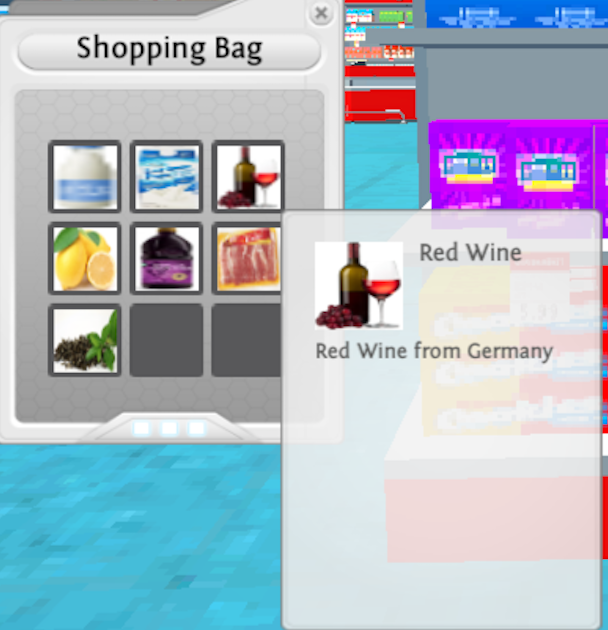
\includegraphics[width=\columnwidth]{ShoppingBag.png}
    \caption{Shows the Shopping Bag and the tool tip of the items.}
    \label{fig:ShoppingBag}
\end{figure}

The game finish if the times runs out or the players goes to the till. In the end he gets points for each correct item he has picked up and a bonus for the leftover time.

In the End the Player got his accomplished points shown and can jump back to the menu to pick a different level. 



%Ideally the chosen tasks would be individual levels which depend on each other and will tell a small story, like car driving → food shopping → cooking.
%The user can either choose the disease for the level himself or a random disease is selected in the beginning.
%The chosen disease should become worse over the time (within one level or across levels) but, if possible and accurate (neglecting the time), the user should also be able to slow down the process or even heal the disease completely.
%Therefore he/she has to take the appropriate measures for the specific disease.
%In order to convincingly convey the topic, using a VR device like the Oculus Rift or an mobile phone / Google Cardboard combination would be beneficial to the project.

\subsection{Diseases}

As described in \cite{gazedisplays} and \cite{eyediseasesim} effects like
blurry or distorted vision, floaters, and reduced field of view can be
efficiently implemented by using fragment shaders. The individual properties
of the shaders and how to decompose the individual diseases into different
shaders (re-usability) is subject to the first research block. But since this
appears to be a very well researched topic, we're confident that we won't run
into any major difficulties. As closer descriped in section 4 we decided to take the four most common eye diseases in Germany: Colorblindess, Myopia and Hyperopia, Glaucoma and Cataract. The last two are more common for older people but espacilly they are important to regognize as early as possible. 

%\begin{table}
%    \textbf{Glaucoma}\\
%    Sudden eye pain, blurred vision and loss of vision especially in the
%    outer regions.
%
%    \vspace{1em}\textbf{Cataracts}\\
%    Blurred vision especially in the center region.
%
%    \vspace{1em}\textbf{Diabetic Retinopathy}\\
%    Black spots in the view.
%
%    \vspace{1em}\textbf{Color blindness}\\
%    Some colours appear indistinguishable.
%
%    \vspace{1em}\textbf{Achromatopsia}\\
%    (Almost) No color sensitivity at all.
%
%    \vspace{1em}\textbf{Myopia / Hyperopia}\\
%    Commonly known as nearsightedness and farsightedness respectively.
%
%    \vspace{1em}\textbf{Kreatoconus}\\
%    The cornea deforms into a conical shape.
%    Multiple ghost images may be visible, arranged in a chaotic pattern,
%    the vision becomes blurry, and visual acuity decreases at all distances.
%    Poor night vision, photo-phobia, and eye strain are additional symptoms.
%
%    \vspace{1em}\textbf{Nyctalopia / Hermalopia}\\
%    High difficulty to see in relatively low and bright light respectively.
%
%    \vspace{1em}\textbf{Retinal detachment / Posterior vitreous detachment}\\
%    Flashes of light, very brief in the extreme peripheral region.
%    Sudden increase in the amount of floaters.
%    Slight feeling of heaviness in the eye.
%    \caption{Eye diseases}
%    \label{tab:eye_diseases}
%\end{table}

\section{The human eye}
Since eye diseases are supposed to be simulated in a virtual environment this section begins with a brief overview over the human eye in comparison to man-made cameras and their abstraction of the pinhole camera used in modern computer graphics.

As can be seen in \Fref{fig:humaneye} the human eye is a spherical shaped organ letting light enter through the pupil to form an image of the world at the retina.
This hole consists of the cornea, the pupil and the lens which act as an objective enabling the eye to focus on various distances and adapt to bright and dark scenes.

The cornea is a transparent layer with a rather fixed shape and therefore a fixed refractive index.
It focuses the light on the pupil which prevents too much light from entering the eye like an aperture.
The lens finally focuses the light on the retina by altering its shape which effectively changes its focal length.
So unlike in cameras focusing is not achieved by altering the distance of the lenses to the sensor but by altering the focal length.

The retina is photosensitive tissue at the back of the eye consisting of rods and cones.
Cones are responsible for color vision and operate in daylight light conditions whereas rods are more light sensitive and provide gray-scale night vision.
But unlike camera sensors, where red, green, and blue pixels are evenly distributed, the retina has a in-homogeneous layout.

There is the macula, which is an area with a very high rod and cone density.
The central part of the macula is called the fovea which consists solely of tightly packed cones.
Compared to the macula, the rest of the eye, however, has a fairly low resolution and mostly consists of the non-color sensitive rods.


\begin{figure}
    \centering
    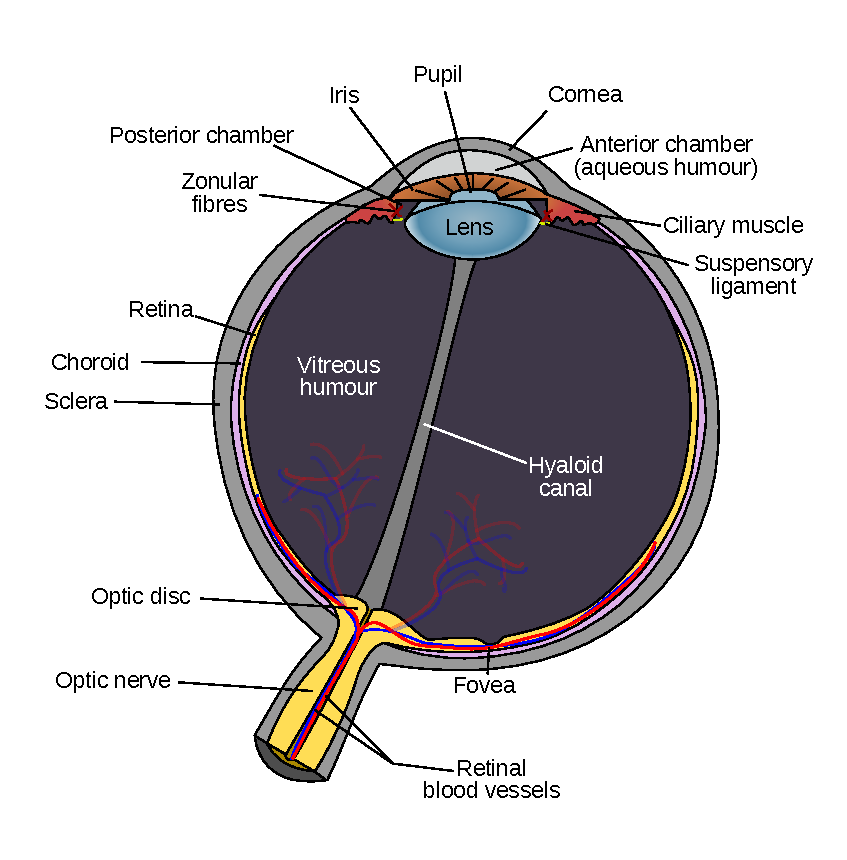
\includegraphics[width=\columnwidth]{human_eye_scheme.pdf}
    \caption{Scheme of the human eye.}
    \label{fig:humaneye}
\end{figure}
%
%
\subsection{Colorblindness}
A first step in simulation color vision deficiency is to understand what color actually is and how humans perceive it.
At first color is nothing than an illusion created in our brain.
From a physical point of view, light can be thought of a wave and therefore described by the waves spectral intensities $\ell(\lambda)$.
Light hitting the rods and cones stimulates them differently based on the wavelength of the incoming light.
This can be described by responsivity curves which.
For the three cone types $L$, $M$, and $S$ of the human eye they are denoted by $\bar l$, $\bar m$, and $\bar s$ and were first determined by a color matching experiment in 1931.
They were used to define the CIE XYZ 1931 color space and are known as the CIE 1931 2º standard observer.\footnote{
    Actually those functions were transformed to have nice properties such as being non-negative.
    As a consequence the base vectors of the resulting XYZ color space describe colors which have no physical representation.
    The color space based on the actual responsivity curves $l$, $m$, and $s$ is called the LMS color space.
    There is a change of basis matrix available to switch from one to the other.
    So let's assume LMS and XYZ to be the same for now.
}

Given a spectral power distribution $\ell$ of a light source, its XYZ color value, also called \emph{tristimulus}, can be computed by the following equations:
%All other color spaces, like the sRGB color space, are defined based on the CIE XYZ 1931 color space or at least provide a mapping to it.
\begin{eqnarray}
    X &= \int\bar x(\lambda) \ell(\lambda) \\
    Y &= \int\bar y(\lambda) \ell(\lambda) \\
    Z &= \int\bar z(\lambda) \ell(\lambda).
\end{eqnarray}
%
Color vision deficiency originates from abnormal cone responses or the absence of one or more cone types.
People missing one of the $L$-, $M$-, or $S$-cones entirely are called \emph{Protanopes}, \emph{Deuteranopes}, and \emph{Tritanopes} respectively.
If all cone types are present but one of them is abnormal in its response, it is referred to as \emph{Protanomaly}, \emph{Deuteranomaly}, and \emph{Tritanomaly} respectively.

The idea of simulating color vision deficiencies is to mimic these changes by first approximating the original spectral power distribution and then computing the new color value based on altered responsivity curves.
Luckily this can be expressed by a linear mapping and therefore be efficiently implemented by means of a matrix multiplication.

So the process of 

\todo{Move this to the beginning of the section or to related work.}
There is already a color blindness simulation available in the Unity Asset store based on Brettel \etal~\cite{brettel}.
However, they focused on Protanopia and Deuteranopia since these are the most common forms.
Machado \etal~\cite{Machado2009} improved this approach by introducing a model for anomalous cones and trying to take the opponent-stage model into account.

In the game, both approaches can be experienced.
We extended the existing asset by the model proposed by Machado by writing a new shader which implements their approach.

%$\bar x$, $\bar y$, and $\bar z$ define a subspace.
%Let $\bar u$, $\bar v$, and $\bar w$ be an orthonormal basis of this subspace with a change of basis matrix $B$.

\begin{figure}
    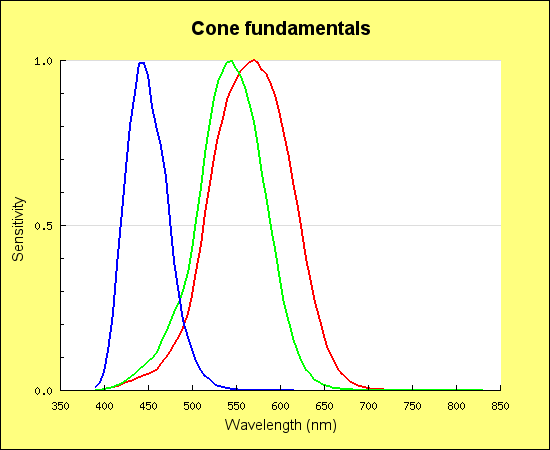
\includegraphics[width=\columnwidth]{lms-sensitivity.png}
    \caption{CIE 2º LMS spectral sensitivity functions~\cite{cvrl-lms-web}.}
    \label{fig:lmscurves}
\end{figure}

\subsection{Glaucoma}

Glaucoma is one of the diseases which damages the optic nerves from the eyes. The result of this is a loss of vision and in the end causing total blindness. 

Several studies shown that the eye pressure is the main factor of an optic nerve damage. By Glaucoma the pressure in the eye is too high that the optic nerve gets damaged. Another factor is the blood pressure, this also can in fact the optic nerves.

How much pressure the optic nerves can tolerate is different for each person. So that is why you cant directly say at witch pressure the optic nerves get damaged.

Glaucoma is especially a problem for people with a family history of glaucoma. Or everybody over the age of 60. In case of Africans or Americans the risk is already getting higher at the age of 40.

There are no Symptoms in the beginning, the vision stays normal and it causes no pain. But without treatment, people with glaucoma slowly lose their peripheral vision. That's why people start to see the things at the corner of their vision field badly. That is shown in \Fref{fig:glaucoma}. Over the time the vision field gets smaller and smaller.~\cite{glaucomafacts}

That's why we made a shader which blurred the outer region of the vision. So that is difficult to see items in there outer regions of there vision.

\begin{figure}
    \centering
    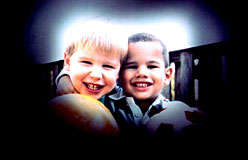
\includegraphics[width=\columnwidth]{glaucomavision.png}
    \caption{Vision of a Person with Glaucoma}
    \label{fig:glaucoma}
\end{figure}

\subsection{Cataract}

Cataract is a disease which effects the lens of the eye. It is clouding the lens and the effect of this is that the person have difficulties to focus on objects and have a different color perception.

The protein in the eye arrange to keep the lens clear and let the light pass. But in the older ages the protein cant clear the lens anymore and they starting to clump together. This is called a cataract. Its starts in small areas of the lens and grow lager over the time. Mostly this starts in the center of the lens. Like shown in \Fref{fig:cataract}.

The Risk of getting cataract is extremely high for people over the age of 80. The percentage for cataract by people over 80 is about 50\%.~\cite{cataractfacts}

Because of the clouding we decided to blur the hole shader a bit and reduce the colors.

\begin{figure}
    \centering
    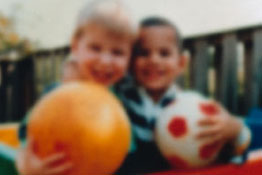
\includegraphics[width=\columnwidth]{cataractvision.png}
    \caption{Vision of a Person with Cataract}
    \label{fig:cataract}
\end{figure}

\subsection{Myopia and Hyperopia}

Myopia and Hyperopia can have different causes. There are \emph{refractive myopia} types which are caused by a changing refractive index of the cornea or lens and there is \emph{axial myopia} which originates in an increased axial length of the eye as seen in \Fref{fig:hyperopia}.
In either case, the focal range of the eye is altered since the lens cannot provide the required focal length for some distances anymore.

\begin{figure}
    \centering
    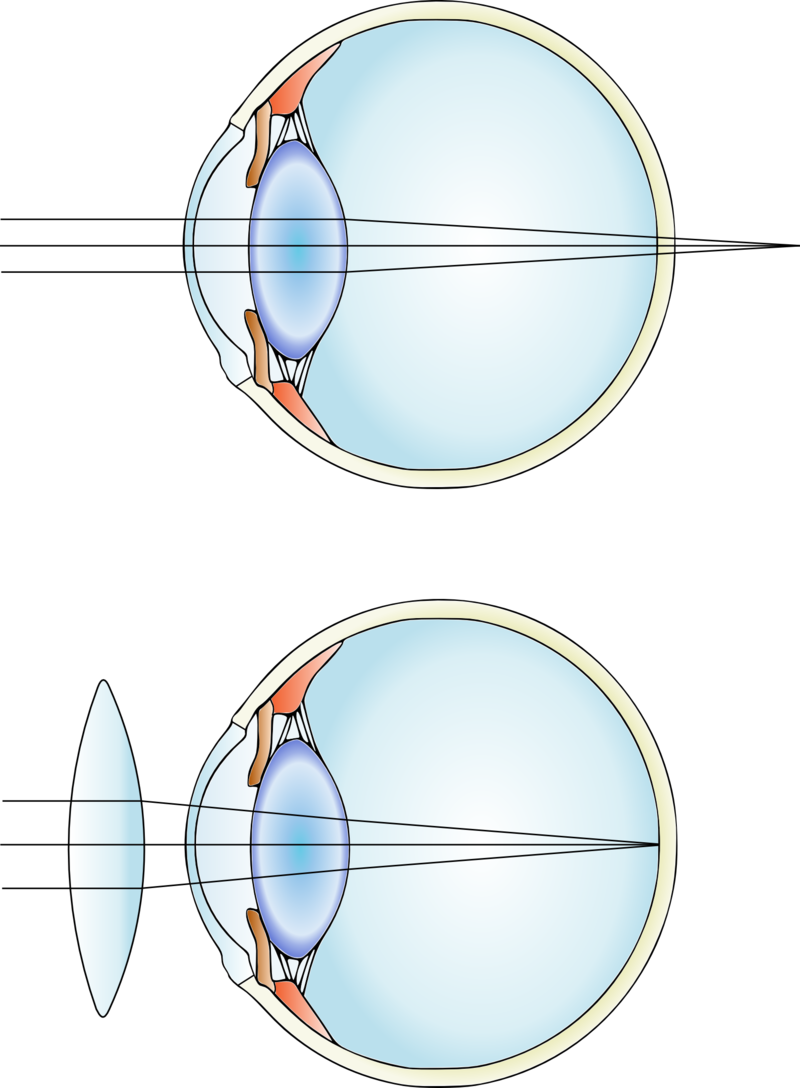
\includegraphics[width=0.75\columnwidth]{hyperopia.png}
    \caption{Hyperotic eye and treatment by glasses.}
    \label{fig:hyperopia}
\end{figure}

In order to simulate that in real-time a simulation of focal depth is needed.
A brief overview can be found at~\cite{gpugems-DoF}.

Unity already provides a fast and decent implementation of real-time focal depth in its Standard Assets.
This was used to simulate axial myopia/hyperopia by limiting the focal distance.

The focal depth asset in Unity has various parameters. Interesting ones are \emph{focal distance}, \emph{aperture}, and \emph{blur size}.
The blur size in combination with the aperture define the maximum blur radius.
The focal distance correlates to the focal length by means of the \emph{thin lens formula}:
\begin{equation}
    \frac{1}{d_p} + \frac{1}{d_I} = \frac{1}{f}.
\end{equation}
Given the cornea-retina distance of 24mm, the focal-length range of the human eye can be estimated by [20,69mm - 24mm] for a distance range from 15cm to ∞.
%
\begin{table}
    \centering
    \begin{tabular}{ll}
        Diopters                & 59-60 dpt \\
        Focal length            & 22-24mm\\
        Pupil diameter          & 2mm - 7/8mm (contracted - dilated) \\
        Cornea-Retina distance  & 17mm/25mm \\
        f-stop                  & ~f/3.2 or f/3.5 \\
        Cone of visual attention& ~55º \\
        Macula                  & 6mm radius, $\sim$150000 px/mm²\\
    \end{tabular}
    \caption{Properties of the human eye~\cite{eye-focal, eyeascamera}}
    \label{tab:eyeproperties}
\end{table}


\section{Project Requirements}

In the following section its written, how the four Project Requirements where implemented.

\subsection{Science}

The game was build CoSMoS compliant especially the different diseases where discovered,modeled. After wards we Tested the different effect of it and documented it in the end. All models base on a scientific background as far as possible. The settings show a specific state of the disease, these stats where so selected that the effect is visible.

\subsection{Gamification}

The player can move free in the supermarket. He gets guidance in form of a text field in the left corner, how he can move, pick up items or open his bag. The part of the game is to find all the required items and beat the time.

\subsection{Complexity}

Through the different eye diseases, its every time a new challenge to find the right objects. These will be the one of the main learning effect the other one is to learn with the info texts about the diseases can be recognize and what to do against it.

\subsection{Aesthetics}

The design of the game is hold quite simple that everybody can quickly understand what to do. All Text fields where set in the corners to give the player the option to fully see the influences of the diseases. Its as far we found the first accessible 3D simulation with a game component.

The player can get more information of each disease in the menu.

%
%
\section{Summary \& Future Work}

Add more of eye diseases like Kreatoconus,Retinal detachment / Posterior vitreous detachment or Diabetic Retinopathy. The diseases could change over the time the game runs. Aswell it would be nice to have more tasks like driving or working to show the effects in different areas.

The Shopping List could get more interactive that it tics stuff of when u got it in your shopping bag.

The hole graphics could be reworked to make it as realistic as possible especially if you using an VR Gadget.

Vinnikov \etal \cite{gazedisplays} developed a Gaze-Contingent-Display in order to evaluate the users eye direction and adept the displayed images in real-time.
Because the effects of eye diseases follow the eye movement, i.e. are static with respect to the eye coordinate frame, they achieved more realistic results in comparison to rendering gaze-independent images.
A consumer solution is under development by the German company SensoMotoric Instruments (SIM) which provides an gaze tracking solution update for the Oculus Rift DK 2 \cite{smi-oculus, arstechoculus}.
According to their website they also provide an integration into various VR engines, including Unity3D, available making it especially interesting for this project.

The gaze-direction would be useful to accurately simulate the vision fields and would also be an interesting human interface for the game mechanics.
%
\printbibliography

\balancecolumns

\end{document}
